\chapter{Metodologia do trabalho}
\label{CAP3}

Esta seção trata das fases do trabalho: como foram  executadas e em que sequência.

% descrever fases do trab: concepcao, projeto, implementacao, testes
% (falar com o prof)


\section{Coleta de dados via celular}
Para coletar dados de aceleração, é possível utilizar os sensores embutidos nos \textit{smartphones}. Através de aplicativos móveis desenvolvidos para este fim, pode-se interagir com os acelerômetros do dispositivo. Esses sensores registram a aceleração em relação a eixos tridimensionais e ortogonais definidos para dispositivos Android, como pode ser visto na figura \ref{fig:axis_android}.


\begin{figure}[hp]
    \centering
    
    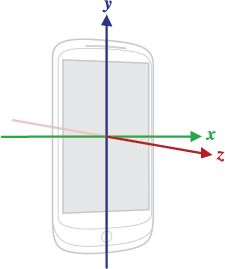
\includegraphics[]{figures/axis_android_device.png}
    
    \caption{Sistema de coordenadas que rege os valores dos acelerômetros de um dispositivo Android\textsuperscript{[27]}.}
    
    \label{fig:axis_android}
\end{figure}

Com o aplicativo desenvolvido, é possível obter informações detalhadas sobre a aceleração do veículo em que o \textit{smartphone} está instalado. A taxa de amostragem desses dados pode ser ajustada para atender às necessidades específicas do sistema por um parâmetro chamado \textit{minMillisBetweenData}, conforme foi definido no repositório do projeto Android no GitHub \textit{GitHub} \url{https://github.com/APF2000/android-obd-reader-pires}. 

Os dados coletados são armazenados e processados para análises posteriores. Os códigos das APIs desenvolvidas para receber as requisições do \textit{app} podem ser encontrados nos Apêndices 7.3 e 7.4 deste documento.

% contribuindo para a avaliação do comportamento de condução e identificação de padrões. Essa abordagem, aproveitando os recursos dos \textit{smartphones}, oferece uma solução prática e acessível para a coleta de dados de aceleração.

A figura \ref{fig:aceleracao} mostra os gráficos da aceleração a partir dos dados coletados do celular. 

% A relação entre o gráfico da aceleração e uma curva feita pelo carro é fundamental para compreender o comportamento dinâmico do veículo durante a condução. No contexto da física do movimento, a aceleração é a taxa de variação da velocidade em relação ao tempo. Quando um carro realiza uma curva, ele experimenta uma aceleração centrípeta, que é direcionada para o centro da curva. Isso significa que a aceleração varia em magnitude e direção conforme o veículo percorre a curva.

% Em um gráfico típico de aceleração durante uma curva, a forma da curva no gráfico pode fornecer informações sobre a suavidade da curva, a intensidade da aceleração lateral e até mesmo indicar a presença de manobras abruptas. Curvas suaves geralmente se refletem em padrões de aceleração mais graduais, enquanto curvas mais acentuadas ou manobras rápidas podem resultar em picos agudos no gráfico.

% Essa relação entre o gráfico de aceleração e a curva feita pelo carro é valiosa não apenas para entender a dinâmica do veículo, mas também para avaliar a qualidade da condução. O Sistema de coleta de informações de veículos que incorporam a análise desses dados podem oferecer \textit{insights} importantes sobre o estilo de direção, ajudando na identificação de comportamentos agressivos, curvas perigosas ou necessidade de aprimoramento nas habilidades de condução. 

% Essa integração contribui para a segurança e eficiência do sistema de rastreamento, proporcionando uma compreensão mais completa do desempenho do veículo em diferentes cenários de condução. A figura \ref{fig:sudden_acc_car} ilustra como essa análise pode ser feita.

\begin{figure}[hp]
    \centering
    
    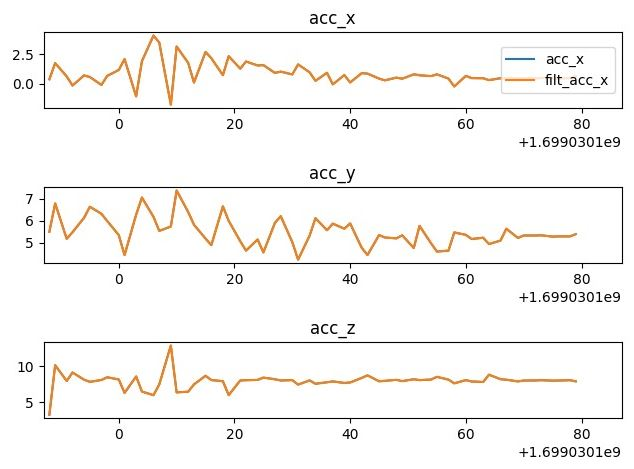
\includegraphics[scale=0.8]{figures/acelaracao.jpg}
    
    \caption{Gráfico da aceleração nos eixos x, y, z.}
    
    \label{fig:aceleracao}
\end{figure}

% \begin{figure}[hp]
%     \centering
    
%     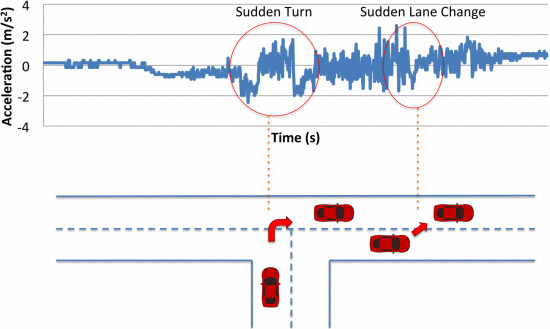
\includegraphics[scale=0.6]{figures/sudden_acc_car.jpg}
    
%     \caption{Correspondência entre variações de aceleração e movimentos relativos do carro\textsuperscript{[15]}.}
    
%     \label{fig:sudden_acc_car}
% \end{figure}

\section{Transferência de dados para a nuvem e estruturação}

A transferência de dados para a nuvem e a sua estruturação desempenham um papel crucial na eficiência e escalabilidade do sistema de rastreamento de veículos. 

Ao adotar-se uma abordagem baseada na nuvem, os dados coletados podem ser transmitidos de maneira eficiente para servidores remotos, centralizando os dados. A estruturação desses dados na nuvem envolve a organização relacional das informações em bancos de dados, possibilitando a recuperação e análise posterior delas. 

% A utilização de serviços de armazenamento em nuvem, no caso de projeto foi utilizado o AWS RDS, permite não apenas a transferência segura dos dados, mas também a flexibilidade de expansão conforme a quantidade de informações aumenta. Assim, a estruturação adequada dos dados na nuvem é fundamental para suportar consultas eficientes, análises e integrações com outras ferramentas, contribuindo para a tomada de decisões informadas e aprimoramento contínuo do sistema de rastreamento de veículos. 

O uso do RDS na nuvem oferece uma solução escalável e resiliente, garantindo que o sistema possa crescer de maneira sustentável ao longo do tempo.

\section{Geração dos dados}
O \textit{app} desenvolvido foi utilizado para gerar dados para o projeto. Isso foi feito apenas pelos próprios integrantes do grupo, uma vez que a demora no desenvolvimento ao longo do trabalho impossibilitou que houvesse grande diversidade entre as informações coletadas.

A princípio, foi decidido que arquivos \textit{.txt} conteriam as informações coletadas, para acelerar o desenvolvimento. Os documentos gerados nessa fase do projeto podem ser encontrados em uma pasta do GoogleDrive criada para o projeto: \url{https://drive.google.com/drive/folders/1Ho0uEHH8MIrNq_SV59YFZzFHzZr1qgSq?usp=sharing}.

Esses arquivos ainda são salvos durante a execução do \textit{app} final, pois é uma forma de \textit{backup} em caso de falha na \textit{internet}, momento durante o qual nenhum dado poderia ser armazenado na nuvem.

A figura \ref{fig:rota} ilustra uma das viagens feita para provar o funcionamento do sistema.

\begin{figure}[hp]
    \centering
    
    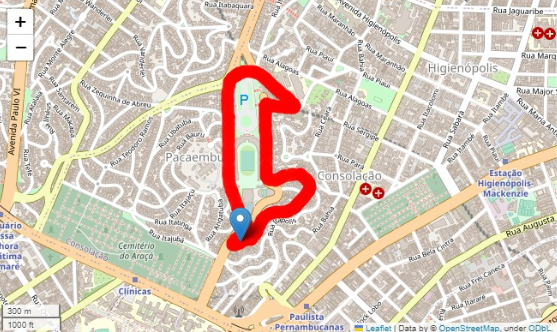
\includegraphics[scale=0.6]{figures/rota.png}
    
    \caption{Rota feita por um dos integrantes do grupo ao redor do seu bairro.}
    
    \label{fig:rota}
\end{figure}

\section{Visualização dos dados}
A análise de dados no contexto deste projeto pode ser eficientemente conduzida utilizando um Jupyter Notebook (exetnsão \textit{.ipynb}). Ao importar os conjuntos de informações coletadas pelo sistema para esse tipo de arquivo, é possível explorar, visualizar e interpretar os dados de maneira flexível, como pode ser visto no repositório onde a análise dos dados foi feita: \url{https://github.com/APF2000/data-analysis}. 

% A variedade de bibliotecas de análise de dados em Python, como Pandas, NumPy e Matplotlib, podem ser aplicadas para realizar operações estatísticas, identificar padrões de comportamento do motorista e gerar visualizações informativas. 

Os Notebooks gerados foram, no entanto, apenas rascunhos para o que viria a seguir no projeto: o desenvolvimento do arquivo \textit{ride\_parser.py}, que é o responsável por transformar em gráficos e tabelas as informações armazenadas no banco de dados.

A API que gera o relatório final sobre o motorista em questão faz uso desse módulo e seu código fonte encontra-se no Apêndice 7.4.

% Dessa forma, o Jupyter Notebook emerge como uma ferramenta essencial para a compreensão aprofundada dos dados coletados, contribuindo significativamente para \textit{insights} valiosos no contexto do sistema de rastreamento de veículos.

\section{Análise dos dados}
Conforme o artigo citado anteriormente, é possível usar métricas de movimentação brusca do carro para classificar motoristas segundo a segurança de sua direção\textsuperscript{[15]}.

Mais especificamente, o estudo determina quatro tipos de condutores: muito cautelosos, cautelosos, agressivos e muito agressivos\textsuperscript{[15]}.

A classificação depende basicamente de quantos movimentos bruscos são feitos e em que situações eles ocorrem. Isso significa que em um ponto de maior convergência de estradas, por exemplo, haverá maior penalidade para o \textit{driver safety index} que em um local de menos movimento ou.

Dessa forma, esse estudo procura ranquear melhor os motoristas que têm menos probabilidade de gerar acidentes.

Inspirado nesse outro trabalho, o grupo focou em gerar métricas qualitativas para perfilar motoristas.

% Inspirados por trabalhos anteriores, o grupo direcionou seus esforços para a geração de métricas qualitativas, visando perfilar os motoristas com base nos padrões identificados nos dados. Essa abordagem permitiu uma análise mais aprofundada do comportamento de condução, proporcionando insights valiosos para aplicações relacionadas à segurança veicular e otimização do desempenho automotivo.

A análise dos dados foi feita através de um processo cuidadoso de tratamento e integração de informações provenientes de diferentes fontes, incluindo os dados do sistema de diagnóstico a bordo (OBD), os dados de aceleração e os dados de GPS (provindos do celular). Inicialmente, esses conjuntos de dados foram processados individualmente para serem salvos em suas próprias tabelas (\textit{DataFrames} na terminologia da biblioteca \textit{pandas} do Python).

Posteriormente, geraram-se metadados de direção apontados por alguns estudos como sendo os mais relevantes para explicar incidentes com um carro (sejam assaltos ou eventos de freada brusca), como era o objetivo inicial do trabalho.

% Os dados provenientes do OBD foram especialmente relevantes, pois forneceram insights cruciais sobre o desempenho do veículo, como o estado do motor e parâmetros de funcionamento. A análise desses dados foi essencial para compreender o comportamento do veículo e extrair informações significativas sobre a condução.

Uma aplicação adicional que surgiu durante o desenvolvimento do projeto foi a validação das informações do OBD com base nos dados do GPS. Essa abordagem permitiu a calibração e a verificação da precisão dos dados do OBD, em particular no que diz respeito à velocidade do veículo.

Utilizando-se as mudanças na latitude e longitude ao longo do tempo, foi possível calcular indiretamente a velocidade do veículo. Isso proporcionou uma maneira de corroborar ou ajustar a velocidade fornecida pelo OBD, garantindo maior confiabilidade nos resultados obtidos e abrindo margem para futuras redundâncias no sistema.

Contudo, é importante destacar uma ressalva em relação aos acelerômetros utilizados. Observou-se que a componente de aceleração na direção do movimento do veículo nem sempre correspondia adequadamente à variação da velocidade obtida pelo GPS. Essa discrepância levantou questões sobre a precisão dos acelerômetros ou sobre possíveis interferências externas que poderiam afetar a medição da aceleração.

\section{Simulador de OBD}
O uso de um simulador de OBD, da marca Freematics, foi necessário durante o desenvolvimento do projeto, uma vez que a disponibilidade de carros para teste esteve quase sempre escassa.

O aparelho usado emula as funcionalidades de um veículo, o que permitiu que o grupo pudesse testar o sistema desenvolvido sem a necessidade de um carro real.

Ademais dessa necessidade inicial do projeto, o simulador é extremamente importante, pois, ao emular dados típicos como velocidade, rotações por minuto (RPM), temperatura do motor, e outros parâmetros do OBD, cria-se um ambiente controlado para verificar a eficácia do sistema em diferentes cenários de condução. 

Isso possibilita testes abrangentes, desde a coleta de dados até a análise de comportamentos específicos, garantindo a robustez e confiabilidade do sistema.

Além disso, o uso do simulador de OBD permite a realização de testes de maneira repetitiva e consistente, fornecendo dados padronizados para avaliação de desempenho e detecção de possíveis problemas antes da implementação em um ambiente de produção. 